\documentclass{beamer}

\usepackage{pri}

\graphicspath{{./}{figures/}{figures/06-ie-figs/}} 

\subtitle{Information Extraction : An Introduction}

\begin{document}

\maketitle

% ------------------------------------------------------------

\begin{frame}
    \frametitle{Bibliography}
    \begin{block}{}
        \begin{itemize}
        \item \href{https://www.cs.uic.edu/~liub/WebMiningBook.html}{Bing Liu, Web Data Mining - Exploring Hyperlinks, Contents, and Usage Data.} Chapter 9.

        \end{itemize}
    \end{block}
\end{frame}
\begin{frame}
    \frametitle{Bibliography - Articles}
    \begin{block}{}
        \begin{itemize}
        \item AnHai Doan, Raghu Ramakrishnan, and Shivakumar
            Vaithyanathan. Managing information extraction: state of the art
            and research directions. In Proceedings of the 2006 ACM SIGMOD
            international conference on Management of data (SIGMOD '06).
            \url{http://doi.acm.org/10.1145/1142473.1142595}
        \item William W. Cohen. Information Extraction and Integration: an
            Overview. \url{http://www.cs.cmu.edu/~wcohen/ie-survey.ppt}
        \end{itemize}
    \end{block}
\end{frame}

\section{Introduction}

\begin{frame}
  \frametitle{Text-based Applications}
  \begin{itemize}
  \item Free-text, semi-structured, streaming ...
      \begin{itemize}
      \item Web pages, email, news articles, call-center text records, business
          reports, annotations, spreadsheets, research papers, blogs, tags,
          instant messages (IM), ...
      \end{itemize}
  \item High-impact applications
      \begin{itemize}
      \item Business intelligence, personal information management, Web
          communities and social media, Web search and advertising, scientific data management,
          e-government, medical records management, ...
      \end{itemize}
  \item Growing rapidly
  \end{itemize}
\end{frame}

\begin{frame}
  \frametitle{Exploiting Text}
  Two main directions:
  \begin{itemize}
  \item Information Retrieval
  \item \emph{Information Extraction}
  \end{itemize}
\end{frame}

\section{Information Extraction}

\newcommand{\job}[1]{\textcolor<4->{red}{#1}}
\newcommand{\artist}[1]{\textcolor<2->{green}{#1}}
\newcommand{\band}[1]{\textcolor<3->{blue}{#1}}

\begin{frame}
    \frametitle{The Task of  Information Extraction}
    \begin{center}
        \begin{minipage}{.8\linewidth}
            \footnotesize Best known as the \job{drummer} in \artist{Jimi
              Hendrix}'s \band{Band of Gypsys}, \artist{Buddy Miles} also had a
            lengthy solo career that drew from rock, blues, soul, and funk in
            varying combinations. Born \artist{George Miles} in Omaha, NE, on
            September 5, 1947, he started playing the \job{drums} at age nine,
            and joined his father's jazz band the \band{Bebops} as a mere 12
            year old. As a teenager, he went on to play with several jazz and
            R\&B outfits, most prominently backing \job{vocal} groups like
            \band{Ruby \& the Romantics}, the \band{Ink Spots}, and the
            \band{Delfonics}.
        \end{minipage}
    \end{center}
    \begin{visibleenv}<5->
        \begin{center}
            \small
            \begin{tabular}{|l|l|l|}\hline
                \textbf{Artist} & \textbf{Band} & \textbf{Instrument}
                \\\hline\hline
                Jimi Hendrix & Band of Gypsys & \\
                Buddy Miles & Band of Gypsys & drums \\
                Buddy Miles & Bebops & drums \\
                Buddy Miles & Ruby \& the Romantics & vocal \\
                Buddy Miles & Ink Spots & vocal \\
                Buddy Miles & Delfonics & vocal \\\hline
            \end{tabular}
        \end{center}
    \end{visibleenv}
\end{frame}

\section{IE Problems and Tasks}

\begin{frame}
  \frametitle{Many Tasks for Extracting Information}
  \begin{itemize}
  \item Named Entity Recognition and Classification
      \begin{itemize}
      \item E.g. Buddy Miles (person), Band of Gypsys (band), ...
      \end{itemize}
  \item Named Entity Resolution (i.e., Entity Linking)
      \begin{itemize}
      \item Buddy Miles $=$ George Miles
      \end{itemize}
  \item Relationship extraction
      \begin{itemize}
      \item Buddy Miles \underline{played} drums \underline{in} Band of Gypsys
      \end{itemize}
  \item Among others...
  \end{itemize}
\end{frame}

\begin{frame}
  \frametitle{Different Facets of IE}
  \begin{itemize}
  \item Different domains
      \begin{itemize}
      \item News, scientific papers, the Web, ...
      \end{itemize}
  \item Different formatting
      \begin{itemize}
      \item Raw text, web pages, ...
      \end{itemize}
  \item Different coverage
      \begin{itemize}
      \item From very domain specific to general open-domain IE
      \end{itemize}
  \item Different complexity
      \begin{itemize}
      \item From restricted vocabulary to ambiguous NL
      \end{itemize}
  \item Different target data models
      \begin{itemize}
      \item From single records to full relational
      \end{itemize}
  \end{itemize}
\end{frame}

\begin{frame}
  \frametitle{An Example Open-Domain IE Project}
  \centering
  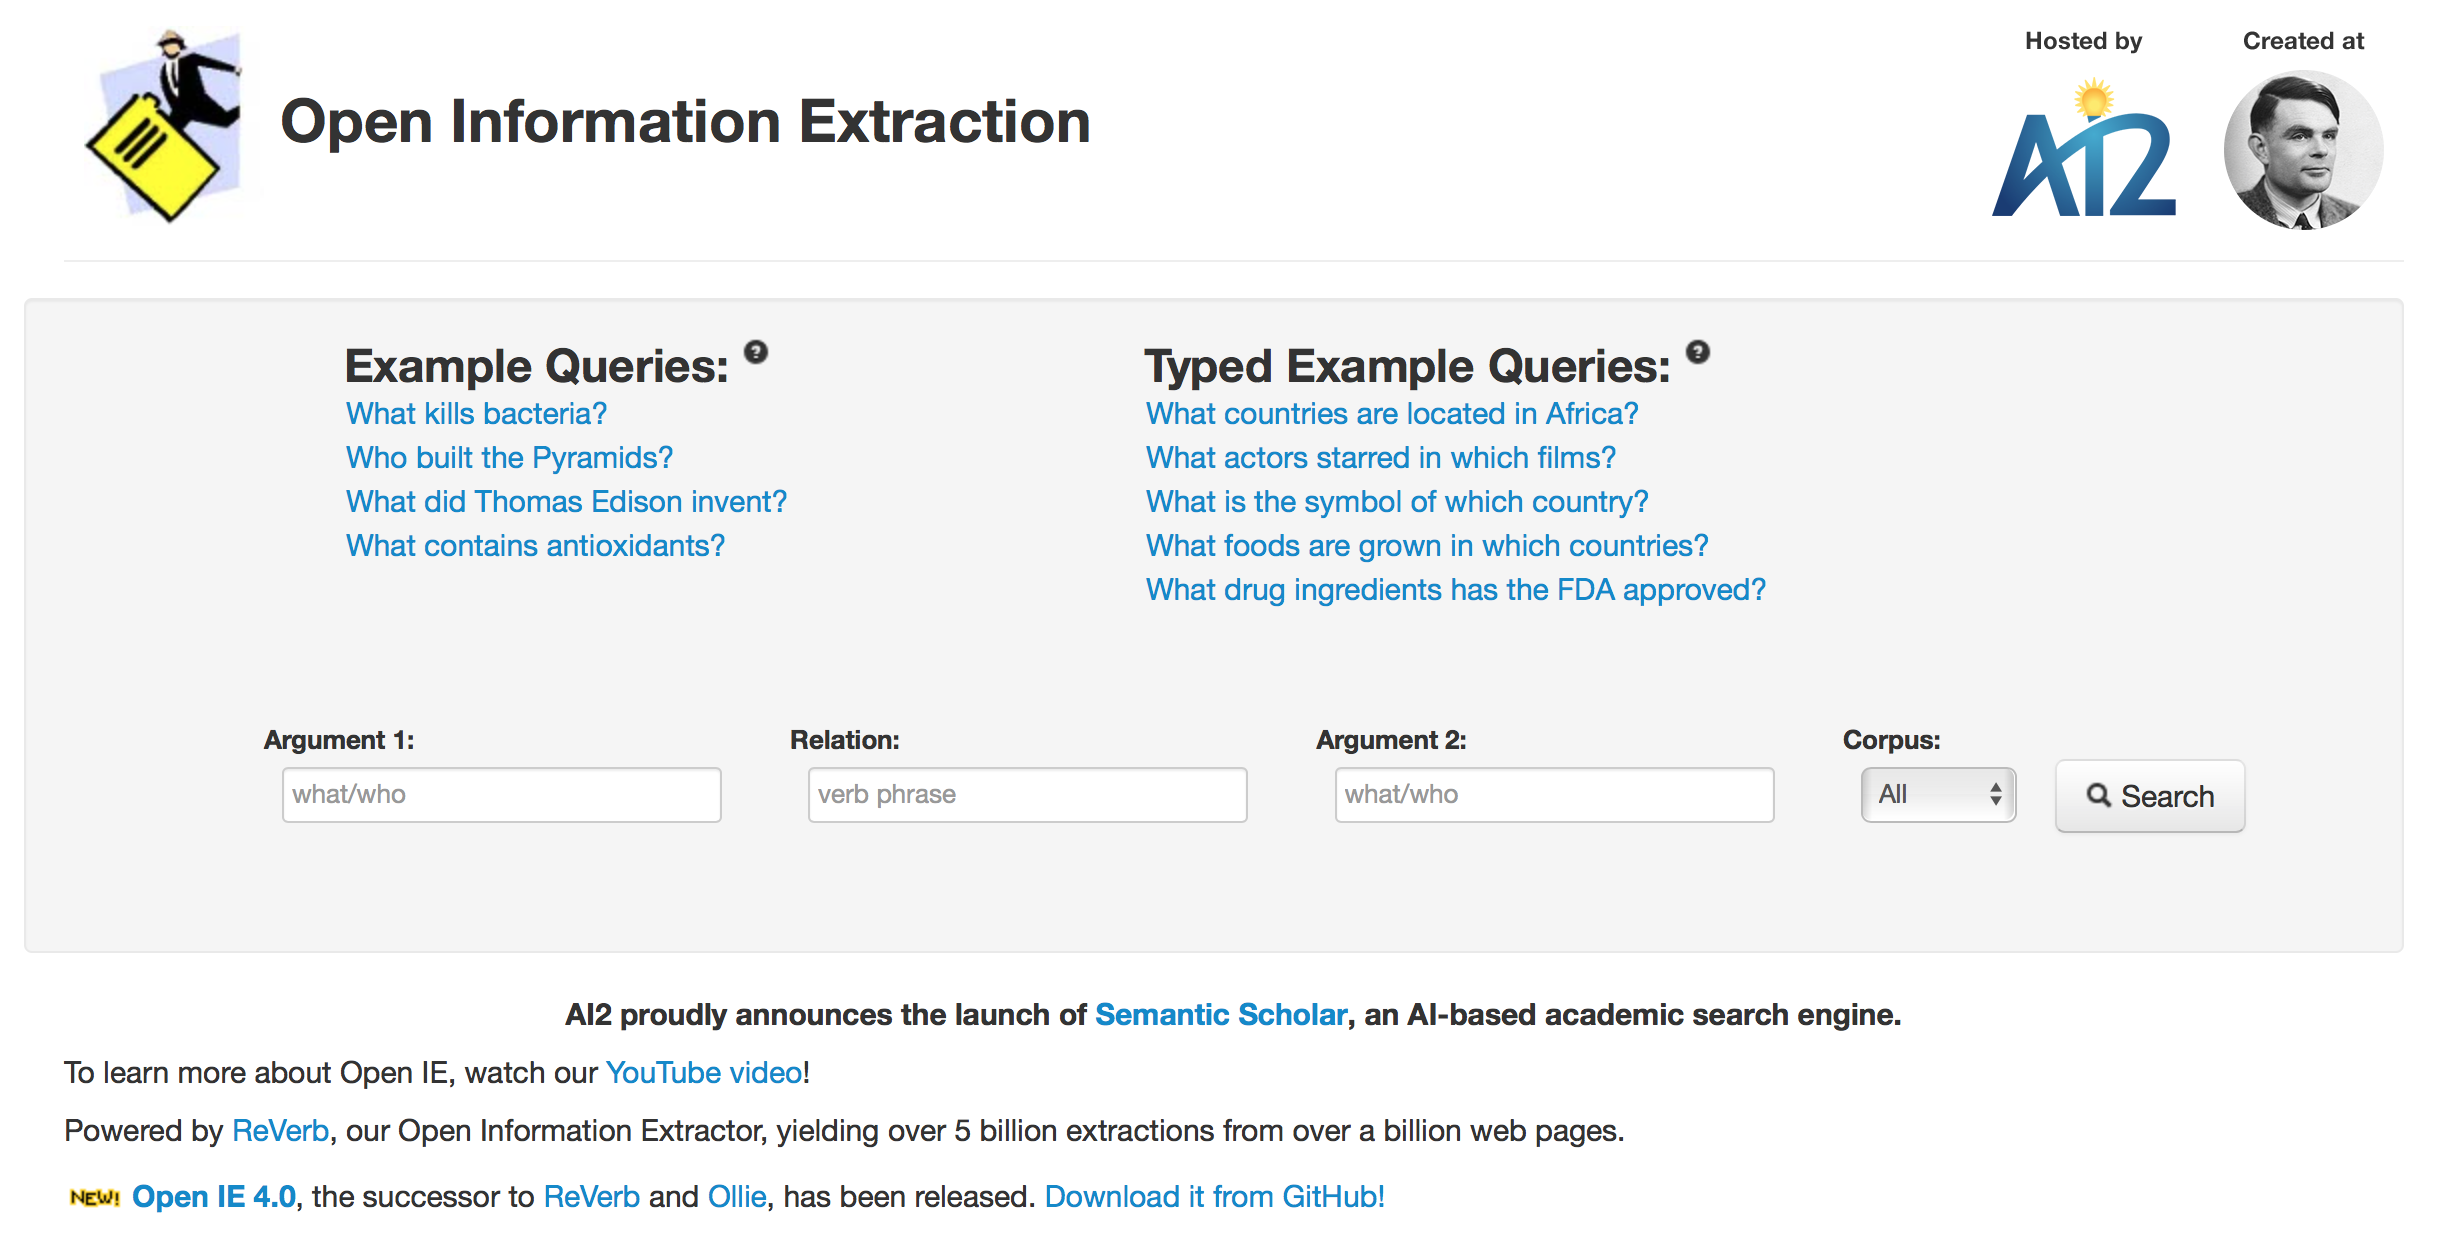
\includegraphics[width=\linewidth]{openie}\\
  \footnotesize\url{http://openie.allenai.org}
\end{frame}

\begin{frame}
  \frametitle{An Example IE Toolkit}
  \centering
  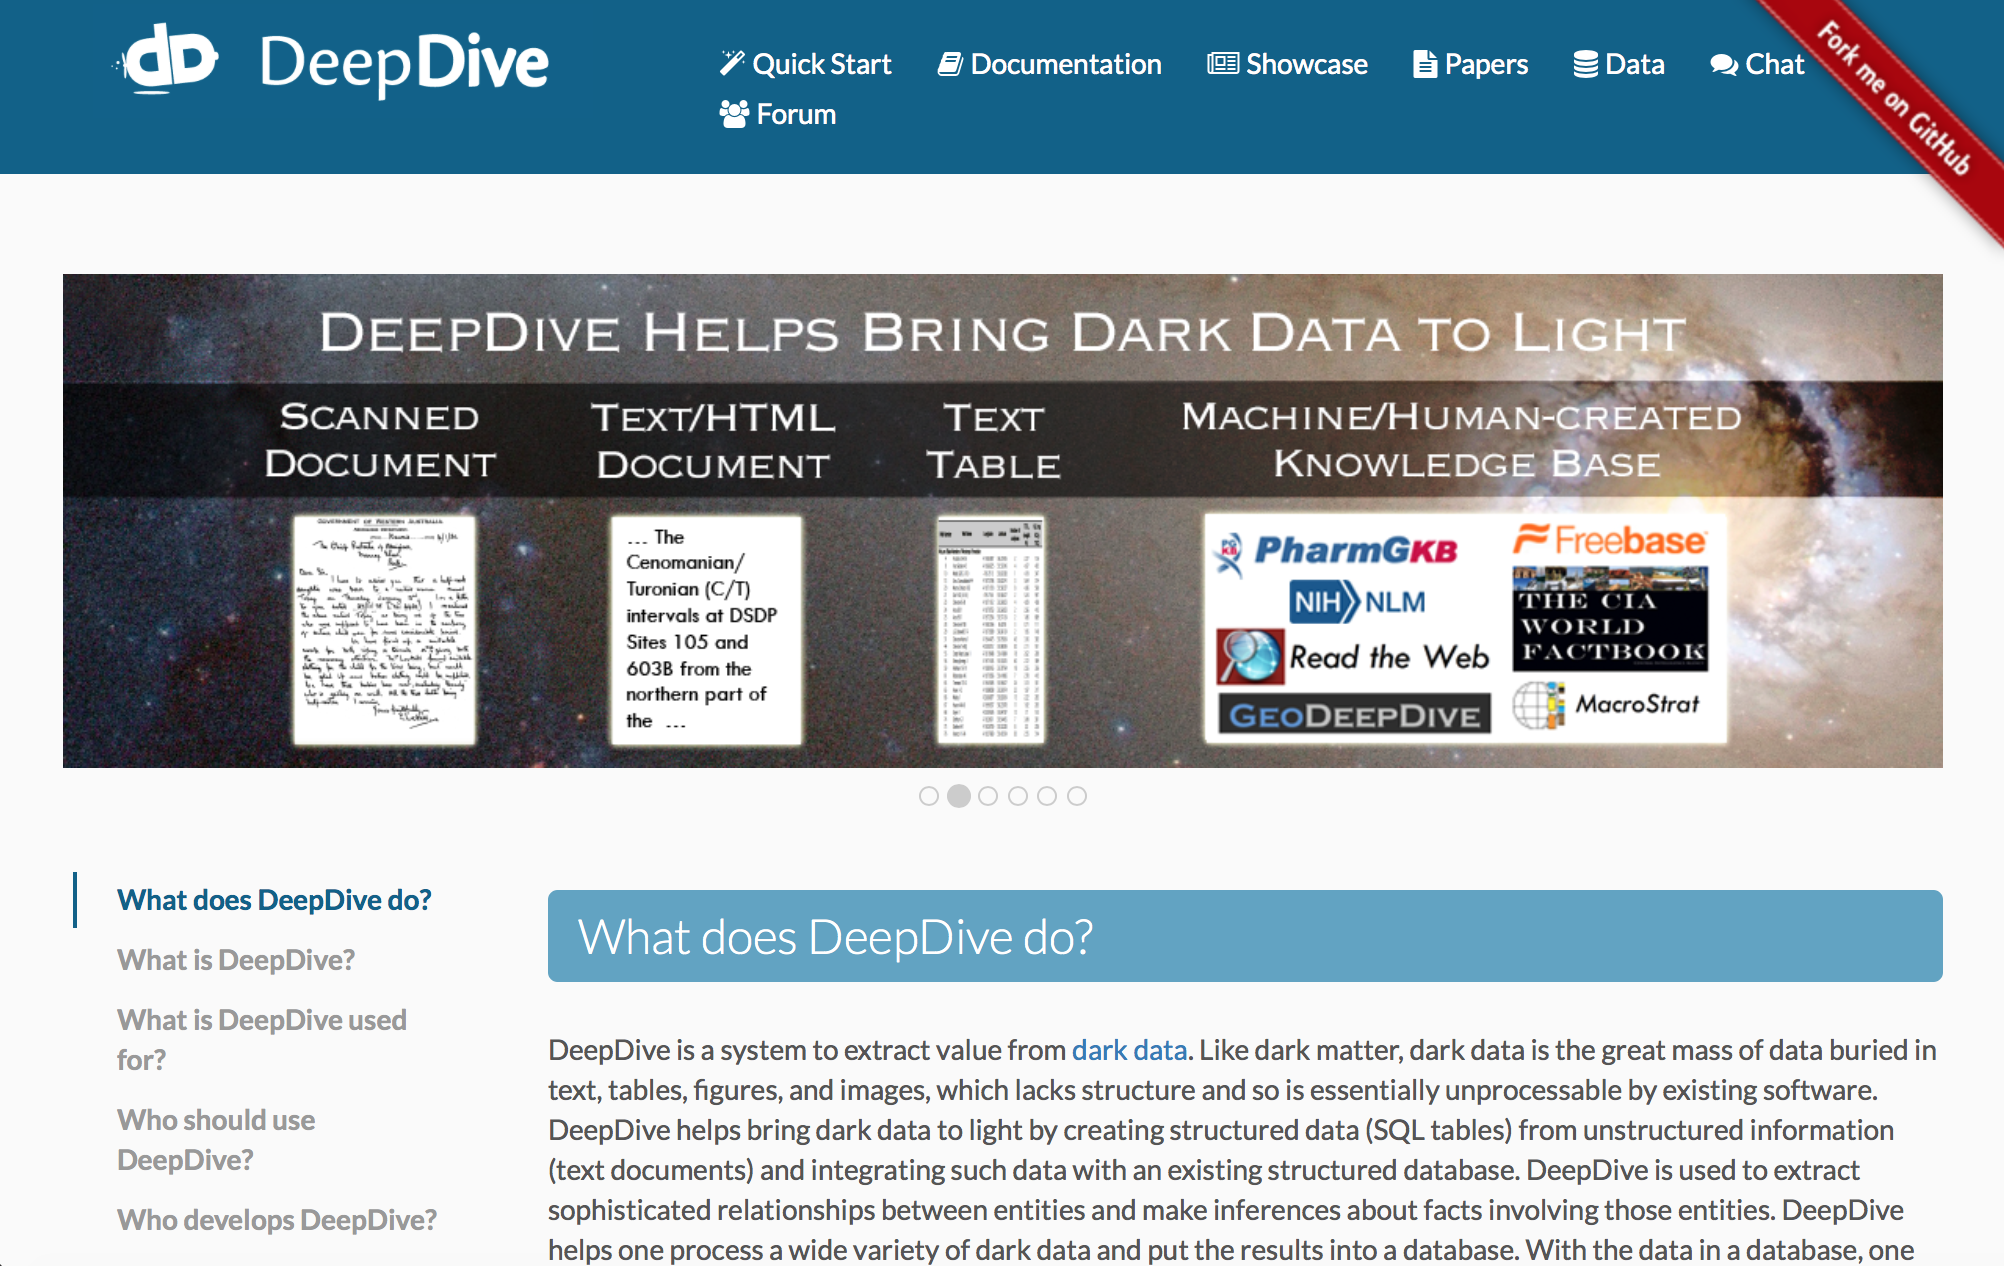
\includegraphics[width=\linewidth]{deepdive}\\
  \footnotesize\url{http://deepdive.stanford.edu/}
\end{frame}

\section{Techniques for IE}

\begin{frame}
  \frametitle{Different Techniques for IE}
  \large
  \begin{block}{}
      \centering
      \begin{minipage}{.65\linewidth}
          \begin{block}{}
              \begin{itemize}
              \item Lexicons
              \item Rules
              \item Classifiers
              \item Sliding Window Classifiers
              \item Sequential Classification Models
              \item Finite State Machines
              \end{itemize}
          \end{block}
      \end{minipage}
      \begin{columns}
          \column{.4\textwidth}
          \begin{exampleblock}{}
              \centering Hand-coded
          \end{exampleblock}
          \column{.4\textwidth}
          \begin{exampleblock}{}
              \centering Machine learning
          \end{exampleblock}
      \end{columns}
      \begin{center}
          Multi-step workflows
      \end{center}
  \end{block}
\end{frame}

\begin{frame}[fragile]
  \frametitle{Example of Hand-coded Rules}
  \tiny
\begin{verbatim}
#############################################################################
# Regular expressions to construct the pattern to extract conference names
#############################################################################
# These are subordinate patterns
my $wordOrdinals="(?:first|second|third|fourth|fifth|sixth|seventh|eighth|ninth|tenth|eleventh|twelfth|thirteenth|fourteenth|fifteenth)";
my $numberOrdinals="(?:\\d?(?:1st|2nd|3rd|1th|2th|3th|4th|5th|6th|7th|8th|9th|0th))";
my $ordinals="(?:$wordOrdinals|$numberOrdinals)";
my $confTypes="(?:Conference|Workshop|Symposium)";
my $words="(?:[A-Z]\\w+\\s*)"; # A word starting with a capital letter and ending with 0 or more spaces
my $confDescriptors="(?:international\\s+|[A-Z]+\\s+)"; # .e.g "International Conference ...' or the conference name for workshops (e.g. "VLDB Workshop ...")
my $connectors="(?:on|of)";
my $abbreviations="(?:\\([A-Z]\\w\\w+[\\W\\s]*?(?:\\d\\d+)?\\))"; # Conference abbreviations like "(SIGMOD'06)"
# The actual pattern we search for. A typical conference name this pattern will find is
# "3rd International Conference on Blah Blah Blah (ICBBB-05)"
my $fullNamePattern="((?:$ordinals\\s+$words*|$confDescriptors)?$confTypes(?:\\s+$connectors\\s+.*?|\\s+)?$abbreviations?)(?:\\n|\\r|\\.|<)";
############################## ################################
# Given a <dbworldMessage>, look for the conference pattern
##############################################################
lookForPattern($dbworldMessage, $fullNamePattern);
#########################################################
# In a given <file>, look for occurrences of <pattern>
# <pattern> is a regular expression
#########################################################
sub lookForPattern {
my ($file,$pattern) = @_;
\end{verbatim}
\end{frame}

\begin{frame}
  \frametitle{An Example IE System Based on Rules}
  \centering
  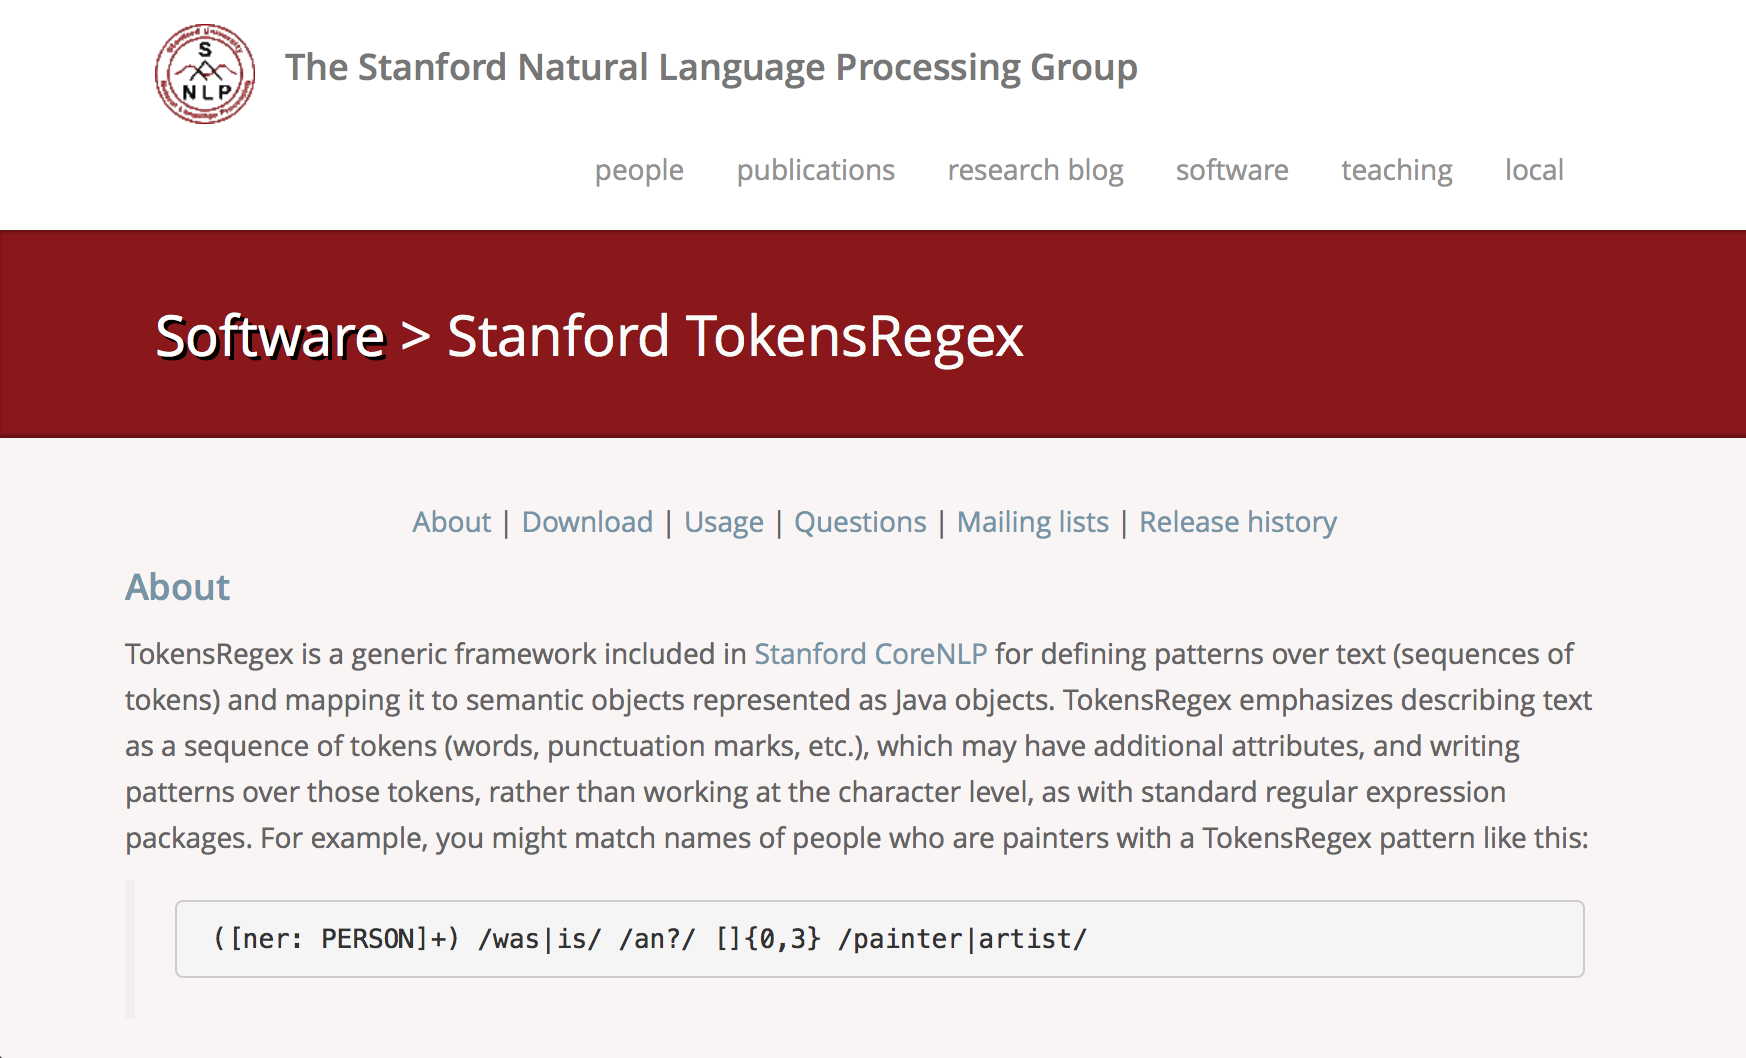
\includegraphics[width=\linewidth]{tokensregex}\\
  \footnotesize\url{http://nlp.stanford.edu/software/tokensregex.html} \\and\\ \url{http://nlp.stanford.edu/software/regexner.html}
\end{frame}

\begin{frame}
\frametitle{Regular Expressions}
Many IE systems based on rules leverage regular expressions!


~\\

Regular expressions are a simple language for searching texts:  
\begin{itemize}
\item Count mentions of a person
\item Extract mentions to numeric quantities (e.g., money), temporal expressions, ISBN codes, $\ldots$ 
\item Prepare texts for analysis: Identify where to {\it split} a document (i.e., \emph{tokenization})
\item $\ldots$
\end{itemize}
Provide a quick introduction here, with some examples...
\end{frame}


\begin{frame}
\frametitle{Some Basics (from Jurafsky Slides) } 
\begin{itemize}
\item Disjunctions
\end{itemize}
\begin{center}
\scriptsize
\begin{tabular} {lll} 
\textbf{RE} & \textbf{Match} & \textbf{Example Patterns Matched}\\
{\tt [mM]oney } & Money or money  & ``\underline{Money}" \\
{\tt [abc] } & `a', `b', or `c'  & ``Investing in Ir\underline{a}n" \\
               &                              & ``is d\underline{a}ngerous \underline{b}usiness"\\
{\tt [1234567890]} & any digit &     ``sitting on \$\underline{7}.\underline{5} billion dollars"      \\
   &   & ``\underline{2}\underline{0}\underline{0}\underline{5} and \underline{2}\underline{0}\underline{0}\underline{6}, more than " \\
   &  &   ``\$\underline{1}\underline{5}\underline{0} million  dollars"    \\
{\tt [$\backslash$.] } & A period &`` `Run!', he screamed\underline{.}" 
\end{tabular}
\end{center}
\end{frame}

\begin{frame} 
\frametitle{Some Basics (from Jurafsky Slides) } 
\begin{itemize}
\item Ranges 
\end{itemize}
\begin{center}
\scriptsize
\begin{tabular} {lll} 
\textbf{RE} & \textbf{Match} & \textbf{Example Patterns Matched}\\
{\tt [A-Z]}  & an upper case letter   & ``\underline{R}ep. \underline{A}nthony \underline{W}einer\\
  &    &   (\underline{D}-\underline{B}rooklyn \& \underline{Q}ueens)" \\
{\tt [a-z]}  & a lower case letter &   ``ACORN'\underline{s}" \\
{\tt [0-9]}  & a single digit  & ``(\underline{9}th CD) " 
\end{tabular}
\end{center}
\end{frame}

\begin{frame}
\frametitle{Some Basics (from Jurafsky Slides) } 
\begin{itemize}
\item Negations 
\end{itemize}
\begin{center}
\scriptsize
\begin{tabular}{lll}
\textbf{RE} & \textbf{Match} & \textbf{Example Patterns Matched}\\
{\tt [\^{}A-Z] } & not an upper case letter &  ``ACORN\alert{\underline{'}\underline{s}}" \\
{\tt[\^{}Ss] } & neither `S' nor `s' & ``\alert{\underline{ACORN'}}s" \\
{\tt[\^{}\textbackslash.] } & not a period & `` `\underline{Run!', he screamed}." \\
\end{tabular}
\end{center}
\end{frame}

\begin{frame}
\frametitle{Some Basics (from Jurafsky Slides) } 
\begin{itemize}
\item Optional Characters: {\tt ?}, {\tt *}, {\tt +} 
\end{itemize}
\begin{center}
\scriptsize
\begin{tabular}{lll}
\textbf{RE} & \textbf{Match} & \textbf{Example Patterns Matched}\\
{\tt colou?r } &  Words with {\tt u}  0 or 1 times& ``\underline{color}"  or \\
                   &                                & ``\underline{colour} " \\
{\tt oo*h!}     & Words with {\tt o}  0 or more times & ``\underline{oh!}" or \\
                      &                                                   &   ``\underline{ooh!}" or \\
                       &                                                   &   ``\underline{oooh!}" \\ 
{\tt o+h!} &   Words with {\tt o} 1 or more times & ``\underline{oh!}" or \\
  &                                                   &   ``\underline{ooh!}" or \\
    &                                                   &   ``\underline{oooooh!}" or \\                       
\end{tabular}
\end{center}
\end{frame}

\begin{frame}
\frametitle{Some Basics (from Jurafsky Slides) } 
\begin{itemize}
\item  Wild Cards \alert{{\tt .} } 
\end{itemize}
\begin{center}
\scriptsize
\begin{tabular}{lll}
\textbf{RE} & \textbf{Match} & \textbf{Example Patterns Matched}\\
{\tt beg\alert{.}n} & Any word with ``beg" then ``n" & ``beg\textcolor{blue}{i}n"~or \\
                          &                                            &  ``beg\textcolor{blue}{a}n"~or \\
                          &                                            &  ``beg\textcolor{blue}{u}n"~or \\
                          &                                            &  ``beg\textcolor{blue}{g}n"~(Poor grammar!) 
                          
 \end{tabular}
 \end{center}
 
 \end{frame}

\begin{frame}
\frametitle{Some Basics (from Jurafsky Slides) } 

\begin{itemize}
\item Start of the line anchor \alert{\^{}}, end of the line anchor \alert{\$}
\end{itemize}


\begin{center}
\scriptsize
\begin{tabular}{lll}
\textbf{RE} & \textbf{Match} & \textbf{Example Patterns Matched}\\
{\tt \alert{\^{}}[A-Z] } & Upper case start of line & ``\underline{P}alo Alto" \\
                            &                                                        & ``the town of \textcolor{gray}{P}alo Alto" \\
{\tt \alert{\^{}}[\^{}A-Z] } & Not upper case start of line &      ``\underline{t}he town of Palo Alto" \\
                            &                                                        & ``\textcolor{gray}{P}alo Alto" \\
{\tt \alert{\^{}}.} & Start of line  & ``\underline{P}alo Alto" \\
                            &                                                        & ``\underline{t}he town of Palo Alto" \\
{\tt .\alert{\$} }      & Identify character that ends a line &    ``Wait\alert{\underline{!}}" \\
                              &                                                & ``This is the end\alert{\underline{.}}" \\

 \end{tabular}
 \end{center}                   
\end{frame}

\begin{frame}
\frametitle{Some Basics (from Jurafsky Slides) } 
\begin{itemize}
\item ``Or"~$|$ statements, Useful short hand 
\end{itemize}
\begin{center}
\scriptsize
\begin{tabular}{lll}
\textbf{RE} & \textbf{Match} & \textbf{Example Patterns Matched}\\
(yours)$|$(mine) & Matches``yours" or ``mine" & ``it's either \underline{yours} or \underline{mine}"\\
$\backslash$d  & Any digit  & ``\underline{1}-Mississippi" \\
$\backslash$D  & Any non-digit & ``1\underline{-Mississippi}" \\
$\backslash$s & Any whitespace character & ``1,\underline{ }2"\\
$\backslash$S & Any non-whitespace character & ``\underline{1,} \underline{2}" \\
$\backslash$w & Any alpha-numeric  &  ``\underline{1}-\underline{Mississippi} " \\
$\backslash$W & Any non-alpha numeric & ``1\underline{-}Mississippi"  \\
\end{tabular}
\end{center}
\end{frame}

\begin{frame}
\frametitle{A Quick Example (from Jurafsky Slides) } 
Quick Example to Illuminate Differences: 

A ``simple" example: identify all instances of \alert{{\tt the}}. \pause 

\begin{itemize}
\invisible<1>{\item[-] \alert{{\tt the } }} \pause 
\invisible<1-2>{\item[] Misses capitalized examples} \pause 
\invisible<1-3>{\item[-] \alert{{\tt [tT]he}}} \pause 
\invisible<1-4>{\item[] Returns words that are too long ({\tt theocrat}, {\tt theme} )} \pause 
\invisible<1-5>{\item[-] \alert{[\^{}a-zA-Z][tT]he[\^{}a-zA-Z] }} \pause 
\invisible<1-6>{\item[] Misses the first ``the" in a sentence } \pause 
\invisible<1-7>{\item[-] \alert{(\^{}$|$[\^{}a-zA-Z])[tT]he[\^{}a-zA-Z] } } 
\end{itemize}
\end{frame}

\begin{frame}
  \frametitle{Most Common Machine Learning Techniques}
  \begin{itemize}
  \item Traditional classifiers
      \begin{itemize}
      \item Naïve Bayes, SVM, ...
      \item Often adapted to handling sequences of words (i.e., {\it sliding window approaches})
      \end{itemize}
  \item Sequence Classifiers (i.e., {\it structured predictors})
      \begin{itemize}
      \item \emph{Hidden Markov Models}
      \item Structured Perceptrons
      \item Conditional Random Fields
      \item Recurrent or Convolutional Deep Neural Networks
      \end{itemize}
  \end{itemize}
\end{frame}

\begin{frame}
  \frametitle{IE as Sequence Classification}
\begin{block}{}
Information Extraction tasks such as Named Entity (NE) Recognition can be modeled as a \emph{sequence classification} problem, leveraging a tagging scheme such as B-I-O
\end{block}
\begin{itemize}
\item \emph{B} stands for ``beginning'' (signifies beginning of a NE)
\item \emph{I} stands for ``inside'' (signifies that the word is inside a NE)
\item \emph{O} stands for ``outside'' (signifies that the word is just a regular word, outside of a NE)
\end{itemize}
\begin{block}{}
Infer the most likely sequence of tags (i.e., classes in a sequential structure), for a given sequence of words.
\end{block}
\end{frame}

% ------------------------------------------------------------

\finalframe{Questions?}

\end{document}
